\chapter{Tensor CP Decomposition on Face Recognition Dataset}
\label{appendix-face-results}
\section{Demonstrate tensor CP decomposition by using the face image dataset}
As an intuitive demonstration for the tensor CP decomposition method, we apply tensor CP decomposition on face image data with 1000 face images, with each image having dimension $96$-by-$96$. Thus, the face image data are encoded in a $3$-way tensor of dimension $1000$-by-$32$-by-$32$. Using tensor CP decomposition, we obtain the first $5$ tensor components, which intuitively represent the prominent facial features in the face images: 
\begin{figure}[H]
    \centering
        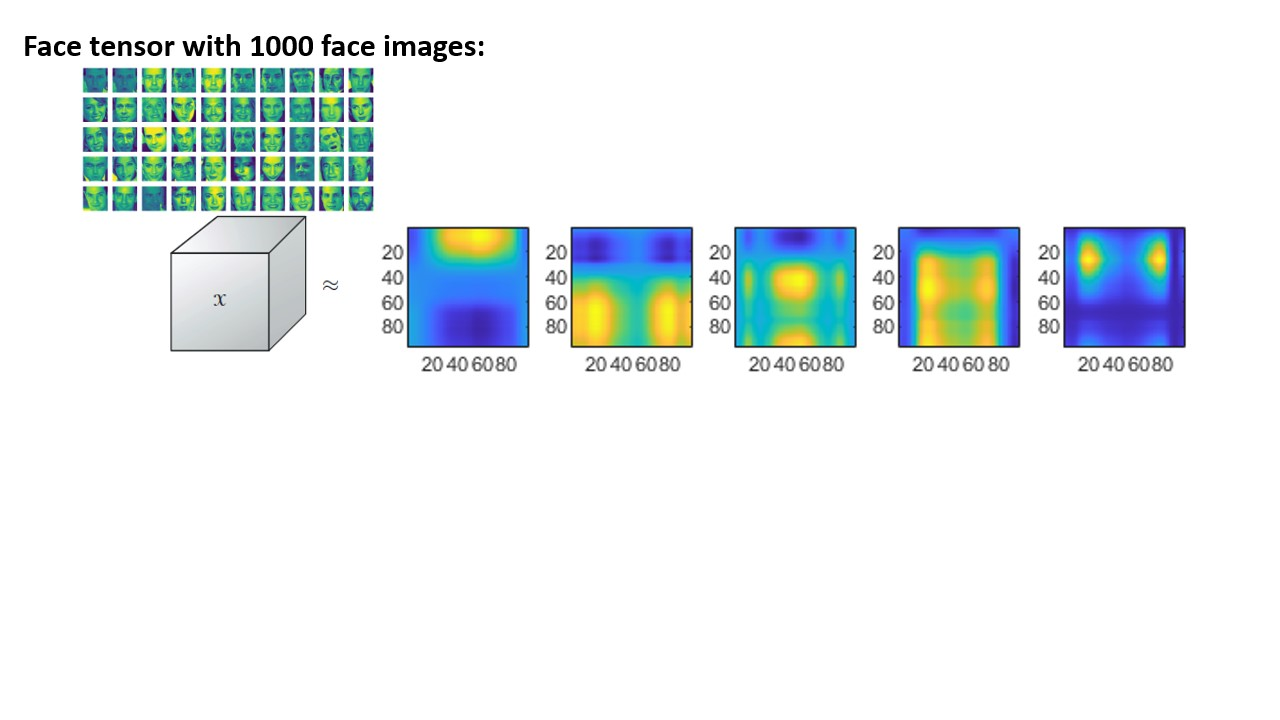
\includegraphics[width=0.7\textwidth]{presentation/Slide2.jpg}
        \caption{First 5 tensor factors for face image data.}
    \end{figure}

By projecting the data onto the first few principal components and apply the $k$-means clustering method, we obtain the following clusters grouped by similar face images: 
\begin{figure}[H]
    \centering
    \begin{subfigure}[b]{0.45\textwidth}
        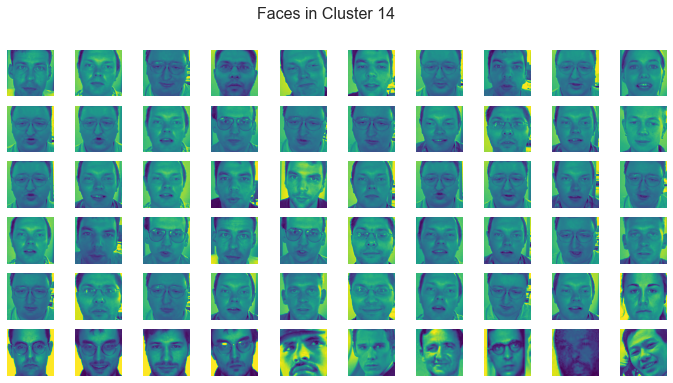
\includegraphics[width=\textwidth]{presentation/figures-face-results/face14.png}
    \end{subfigure}
    \hfill 
    \begin{subfigure}[b]{0.45\textwidth}
        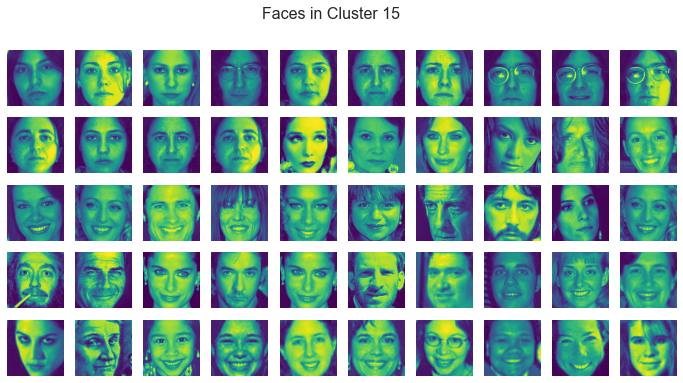
\includegraphics[width=\textwidth]{presentation/figures-face-results/face15.png}
    \end{subfigure}
    \hfill
    \begin{subfigure}[b]{0.45\textwidth}
        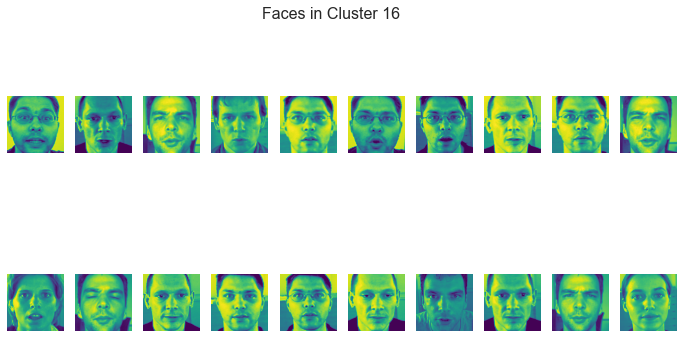
\includegraphics[width=\textwidth]{presentation/figures-face-results/face16.png}
    \end{subfigure}
    \hfill
    \begin{subfigure}[b]{0.45\textwidth}
        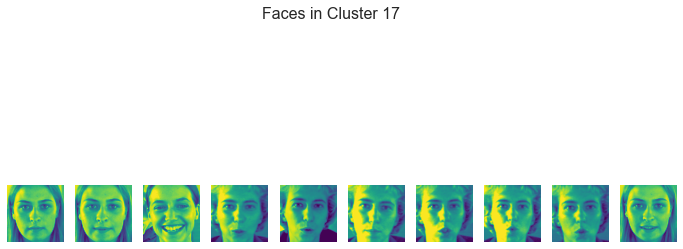
\includegraphics[width=\textwidth]{presentation/figures-face-results/face17.png}
    \end{subfigure}
    \caption{Some arbitrary clusters showing the results of tensor CP decomposition for face data.}
    \end{figure} 
    